\documentclass{book}

\usepackage[utf8]{inputenc}
\usepackage{titlesec}
\usepackage{easylist}
\usepackage{hanging}
\usepackage{hyperref}
\usepackage[a4paper,top=2.0cm,bottom=2.0cm,left=2.0cm,right=3.0cm]{geometry}
\usepackage{blindtext}
\usepackage{tipa}
\usepackage{epigraph}
\usepackage{enumerate}
\usepackage{longtable}
\usepackage{setspace}
\usepackage{verbatim}
\usepackage[T1]{fontenc}
\usepackage{graphicx}
\usepackage[italian]{babel}
\usepackage{amsmath}
\usepackage{pbox}
\usepackage{fancyhdr}
\usepackage{cancel}
\usepackage{tabularx}
\usepackage{booktabs}
\usepackage{multirow}
\usepackage{longtable}
\usepackage{tikz}
\usepackage{tikz-qtree}
\usepackage{subfig}
\usepackage{xcolor}
\usepackage{amssymb}
\usepackage{amsmath}
\usepackage{mathrsfs}
\usepackage{textcomp}
\usepackage{circuitikz}
\usepackage{pifont}
\usepackage{imakeidx}
\usepackage{verbatim}
\usepackage{dsfont}
\usepackage{listings}
\usepackage{color}
\usepackage{upgreek}
\usepackage{tasks}
\usepackage{exsheets}
\usepackage{pgfplots}
\usepackage{lipsum}

\SetupExSheets[question]{type=exam}

\definecolor{mygreen}{rgb}{0,0.6,0}
\definecolor{mygray}{rgb}{0.5,0.5,0.5}
\definecolor{mymauve}{rgb}{0.58,0,0.82}

\lstset{
  backgroundcolor=\color{white},   % choose the background color; you must add \usepackage{color} or \usepackage{xcolor}; should come as last argument
  basicstyle=\footnotesize,        % the size of the fonts that are used for the code
  breakatwhitespace=false,         % sets if automatic breaks should only happen at whitespace
  breaklines=true,                 % sets automatic line breaking
  captionpos=b,                    % sets the caption-position to bottom
  commentstyle=\color{mygreen},    % comment style
  deletekeywords={...},            % if you want to delete keywords from the given language
  escapeinside={\%*}{*)},          % if you want to add LaTeX within your code
  extendedchars=true,              % lets you use non-ASCII characters; for 8-bits encodings only, does not work with UTF-8
  firstnumber=1000,                % start line enumeration with line 1000
  frame=single,	                   % adds a frame around the code
  keepspaces=true,                 % keeps spaces in text, useful for keeping indentation of code (possibly needs columns=flexible)
  keywordstyle=\color{blue},       % keyword style
  language=Octave,                 % the language of the code
  morekeywords={*,...},            % if you want to add more keywords to the set
  numbers=left,                    % where to put the line-numbers; possible values are (none, left, right)
  numbersep=5pt,                   % how far the line-numbers are from the code
  numberstyle=\tiny\color{mygray}, % the style that is used for the line-numbers
  rulecolor=\color{black},         % if not set, the frame-color may be changed on line-breaks within not-black text (e.g. comments (green here))
  showspaces=false,                % show spaces everywhere adding particular underscores; it overrides 'showstringspaces'
  showstringspaces=false,          % underline spaces within strings only
  showtabs=false,                  % show tabs within strings adding particular underscores
  stepnumber=2,                    % the step between two line-numbers. If it's 1, each line will be numbered
  stringstyle=\color{mymauve},     % string literal style
  tabsize=2,	                   % sets default tabsize to 2 spaces
  title=\lstname                   % show the filename of files included with \lstinputlisting; also try caption instead of title
}

\linespread{1.2} % l'interlinea

\frenchspacing

\newcommand{\abs}[1]{\lvert#1\rvert}

\usepackage{floatflt,epsfig}

\usepackage{multicol}
\newcommand\yellowbigsqcup[1][\displaystyle]{%
  \fboxrule0pt
  \ifx#1\textstyle\fboxsep-0.6pt\else\fboxsep-1.25pt\fi
  \mathrel{\fcolorbox{white}{yellow}{$#1\bigsqcup$}}}

\title{Appunti di Reti di telecomunicazioni}
\author{Nicola Ferru}
\date{}
\makeindex[columns=3, title=Alphabetical Index, intoc]

\begin{document}
\maketitle
\tableofcontents
\listoftables
\listoffigures
\chapter{Introduzione}
\chapter{Introduzione}
\label{chap:intro}
\begin{defi}
  GNU/Octave è un applicativo per il calcolo matriciale che consente di svilgere
  tutte le operazioni base e non solo a riguardo, dallo somma, divisione,
  moltiplicazioni e sottrazioni tra matrici, calcolo del determinante, del
  grado e tanto altro.
\end{defi}

\section{Pacchetti e impostazioni base}
\label{sec:packbase}

\subsection{Pacchetti}
\label{sec:pack}

\begin{table}[th]
  \centering
  \begin{tabular}{ll}
    {\bf Nome} & {\bf Descrizione}\\\hline
    \href{https://gnu-octave.github.io/packages/fuzzy-logic-toolkit/}{fuzzy-logic-toolkit} & Un toolkit di logica fuzzy per lo più
                                                                                               compatibile con MATLAB per Octave \\\hline
    \href{https://gnu-octave.github.io/packages/symbolic/}{symbolic} & Aggiunge funzionalità di calcolo simbolico a GNU
                        Octave \\\hline
    \href{https://gnu-octave.github.io/packages/ocs/}{Circuit Simulator (OCS)} & Risolvere equazioni di circuiti elettrici DC e transitori. \\\hline
    \href{https://gnu-octave.github.io/packages/control/}{Control} & Strumenti CACSD ({\it Computer-Aided Control System
                       Design}) per GNU Octave,\\ &basati sulla libreria SLICOT.\\\hline
    \href{https://gnu-octave.github.io/packages/instrument-control/}{instrument-control} & Funzioni I/O di basso livello per interfacce seriali, i2c, parallele, tcp, gpib, vxi11,\\
               &udp e usbtmc.\\\hline 
  \end{tabular}
  \caption{pacchetti utili}
  \label{tab:pachutil}
\end{table}

\subsection{Funzione di identificazione di una variabile}
\label{sec:funiden}
\begin{table}[ht]
  \centering
  \begin{tabular}[tab:funzionediid]{ll}
    {\bf Nome} & {\bf Descrizione} \\\hline
    \lstinline|whos M| & stampa i dati completi sulla variabile
  \end{tabular}
  \caption{Funzione di identificazione}
  \label{tab:funzionediid}
\end{table}
\subsubsection{Stampa a video}
\label{sec:stampiden}
\begin{small}
\begin{verbatim}
Variables visible from the current scope:
variables in scope: top scope
  Attr   Name        Size                     Bytes  Class
  ====   ====        ====                     =====  =====
         M           3x3                         72  double
Total is 9 elements using 72 bytes
\end{verbatim}
\end{small}
\clearpage

\subsubsection{Come funziona}
All'interno di Octave e Matlab sono presenti le classi di variabili
esattamente come accade in altri linguaggi più di programmazione più blasonati,
esso ovviamente è relegato alle funzioni matematiche e grafiche per cui è
pensato il programma.
\begin{figure}[ht]
  \centering
  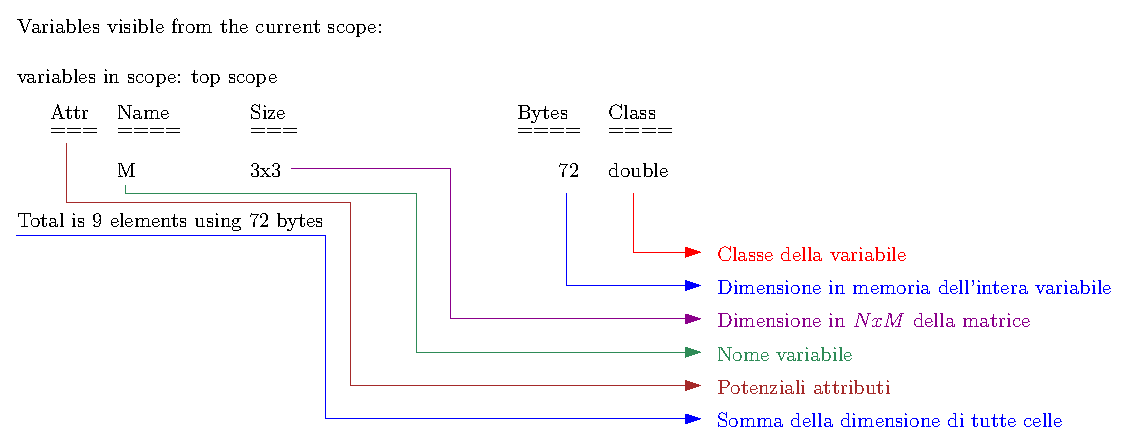
\includegraphics[width=15cm]{img/finiti/whos.eps}
  \caption{descrizione dell'interfaccia di funzione}
  \label{fig:interffun}
\end{figure}
\begin{notab}
  Anche la variabile singola viene vista come una matrice 1x1, da questo si
  denota che come il suo cugino Matlab è un software pensato per elaborare
  prodotti matriciali, infatti, il nome Matlab non sta per \texttt{Mathematic
    lab} ma per \texttt{Matrix Lab}. 
\end{notab}
\subsection{Tipi variabile}
\label{sec:tipivariabile}

\begin{table}[ht]
  \centering
  \begin{tabular}{llll}
    {\bf Nome} & {\bf Descrizione} & {\bf Dimensione} & {\bf Cifre rappresentabili}\\\hline
    \lstinline|double| ({\bf default}) & double-precision array & 8byte & $\pm1.79769x10^{308}$ a $\pm2.22507x10^{-308}$\\\hline
    \lstinline|single| & single-precision array & 4byte & $-2.1475x10^9$ a $2.1475x10^9$\\\hline 
    \lstinline|int8| & Array di interi con segno & 8bit & $-128$ a $127$\\\hline
    \lstinline|int16| & Array di interi con segno & 16bit & $-32768$ a $32767$ \\\hline
    \lstinline|int32| & Array di interi con segno & 32bit & $-2.1475x10^9$ a $2.1475x10^9$\\\hline 
    \lstinline|int64| & Array di interi con segno & 64bit & $-9.2234x10^{18}$ a $9.2234x10^{18}$\\\hline
    \lstinline|uint8| & Array di interi senza segno & 8bit & $255$\\\hline
    \lstinline|uint16| & Array di interi senza segno & 16bit & $65535$ \\\hline
    \lstinline|uint32| & Array di interi senza segno & 32bit & $4.2950x10^9$\\\hline 
    \lstinline|uint64| & Array di interi senza segno & 64bit & $1.8447x10^{19}$\\\hline
  \end{tabular}
  \caption{Tipi variabile}
  \label{tab:tipivariabile}
\end{table}
\begin{oss}
  Questa rapresentazione in memoria vale per la singola cella, quindi bisogna
  moltiplicare il paso per il numero di celle dello stesso tipo. Il programma
  peserà quanto il numero complessivo delle variabili presenti.
\end{oss}

\paragraph{Le stringhe --}
Un altro tipo di variabile però implicita sono le stringhe che il programma può
gestire, nel sequente modo \lstinline|str = "string x"| e la stampa di stringa
viene fatta con un semplice \lstinline|printf(str)|.
\clearpage
\subsubsection{Cosa stampa e cosa no}
Nel linguaggio di Matlab e Octave vengono stampate tutte le associazioni,
funzioni e inizializzazioni che non terminano con il ``{\color{red};}''.

\subsection{Impostazioni e formati}
\label{sec:formImp}
\begin{table}[ht]
  \centering
  \begin{tabular}{lll}
    {\bf Nome} & {\bf Descrizione} & {\bf Visuale}\\\hline
    \lstinline|rat| & Aspetto rateo (invece dei numeri reali rende numeri frazionari) & 1/2\\\hline
    \lstinline|short| & Formato breve a decimale fisso con 4 cifre dopo la virgola. (\textit{default}) & 0.5000\\\hline
    \lstinline|long| & Formato lungo a decimale fisso con 15 cifre dopo la virgola per & 0.500000000000000\\
                     &  i valori doppi e 7 cifre dopo la virgola per i valori singoli. \\\hline
    \lstinline|shortE| & Formato breve in annotazione scientiica con 4 cifre dopo la virgola & 5.0000e-01\\\hline
    \lstinline|longE| & Formato lungo a decimale fisso con 15 cifre dopo la virgola per & 5.000000000000000e-01\\
               & i valori doppi e 7 cifre dopo la virgola per i valori singoli.\\\hline
    \lstinline|shortG| & Formato breve, decimale fisso o notazione scientifica, a seconda & 0.5000\\
               & di quale sia più compatto, con un totale di 5 cifre.\\\hline
    \lstinline|longG| & Formato lungo a decimali fissi o notazione scientifica, qualunque & 0.500000000000000\\
               & sia il più compatto, con un totale di 15 cifre per i valori doppi e\\ & 7 cifre per i valori singoli.\\\hline
    \lstinline|shortEng| & Breve notazione ingegneristica (l'esponente è un
                           multiplo & 500.0000e-003\\
    
               &di 3) con 4 cifre dopo la virgola.\\\hline
    \lstinline|longEng| & Notazione ingegneristica lunga (l'esponente è un multiplo di 3) & 500.000000000000000e-003\\ & con 15 cifre significative.\\\hline
    \lstinline|+|&Formato positivo/negativo con caratteri +, - e vuoti visualizzati & +\\
               & per elementi positivi, negativi e zero.\\\hline
    bank & Formato valuta con 2 cifre dopo la virgola. & 0.50 \\\hline
    hex & Rappresentazione esadecimale di un numero binario & 3fe0000000000000 \\
               & a doppia precisione.\\\hline 
  \end{tabular}
  \caption{Impostazioni e formati}
  \label{tab:form}
\end{table}
\begin{notab}
  È possibile salvare il formato in una variabile con il comando \lstinline|fmt = format("nomeFormato")|
  per poi riutilizzarlo in seguito richiamando \lstinline|format(fmt)|. Altro aspetto esso può cambiare durante lo script quindi è possibile ripotare un dato
  in un formato di stampa e uno in un altro.
\end{notab}

\section{Sistemi di comunicazione}
\subsubsection{Trasmissione}
Sorgente fisica $\to$ Trasduttore $\to$ TX $\to$ Al canale di comunicazione
\subsubsection{Recezione}
Dal canale di comunicazione $\to$ RX $\to$ Trasduttore $\to$ Utente finale
\begin{itemize}
	\item TX = Trasmittente
	\item RX = Ricevitore
\end{itemize}
\subsection{Classificazione di sistemi}
\begin{tasks}(2)
	\task \texttt{Punto-Punto}
	\begin{itemize}
		\item 1 trasmettitore
		\item 1 o più ripetitori intermedi
		\item 1 ricevitore
		\item ad ogni tratta vengono associati uno o più mezzi fisici di
			propagazione del segnale
		\item il canale è una risorsa dedicata al collegamento
	\end{itemize}
	\task \texttt{Multi-utente}
	\begin{itemize}
		\item 1 o più trasmettitori iniziali
		\item 1 o più ripetitori
		\item il canale è una risorsa condivisa tra i diversi trasmettitori e/o
			ricevitori presenti nel sistema
		\item \textit{broadcast} se coinvolge tutti gli utenti come ricevitori.
	\end{itemize}
\end{tasks}
\subsection{Rete di telecomunicazioni}
\begin{itemize}
	\item Piattaforma tecnologica
	\item Obiettivi
		\begin{itemize}
			\item effettuare comunicazione a distanza tra \textit{due} o più
				utenti
			\item trasferire informazione (servizio di telecomunicazioni)
				caratterizzata da diversi parametri (durata, qualità, etc.)
			\item gestire le sue parti componenti e i servizi supportati
		\end{itemize}
	\item Ci sono diverse modalità (e dunque topologie) per realizzare tale
		trasferimento: vantaggi/svantaggi.
\end{itemize}
\subsubsection{Criteri di classificazione di reti}
La classificazione può essere basata su
\begin{enumerate}
	\item gamma dei servizi supportati
	\item grado di mobilità del terminale
	\item estensione fisica
	\item posizione
\end{enumerate}
\subsection{Classificazione per servizi}
\begin{tasks}(2)
	\task Rete \textbf{dedicata} a un servizio
	\begin{itemize}
		\item fornitore di un singolo servizio
		\item possono essere utilizzate con alcune limitazioni anche per un
			insieme ristretto di altri servizi
		\item esempio: la rete telefonica fissa e le prime generazioni di reti
			mobili (GSM)
	\end{itemize}
	\task Rete \textbf{integrata nei servizi}
	\begin{itemize}
		\item fornitura di una vasta gamma di servizi
		\item prestazioni complessive di qualità e di costo decisamente
			migliori rispetto a quella ottenibile con le reti dedicate
		\item esempio: Internet e le reti mobili dalla generazione 2G in poi.
	\end{itemize}
\end{tasks}
\subsection{Classificazione per mobilità}
\begin{tasks}(2)
	\task Rete \textit{fissa}
	\begin{itemize}
		\item gli utenti accedono alla rete da postazioni fisse, oppure si
			muovono in un interno relativamente ristretto
		\item ``punto di accesso'' fisso, terminale può essere mobile
		\item esempio: terminali Wi-Fi che accedono alla rete Internet
	\end{itemize}
	\task Rete \textit{mobile}
	\begin{itemize}
		\item gli utenti possono muoversi senza limitazioni ai loro spostamenti
			(anche tramite veicoli) ``Ovviamente nei limiti prevista dalla
			copertura del ISP''
		\item gli utenti possono cambiare ``punto di accesso'' alla rete che
			gestisce ciò rendendoli sempre raggiungibili (\textit{handever})
		\item esempio: reti cellulari
	\end{itemize}
\end{tasks}
\subsection{Classificazione per estensione}
\begin{tasks}(4)
	\task PAN
	\begin{itemize}
		\item area personale (\textit{circa 1m})
		\item Bluetooth
	\end{itemize}
	\task LAN
	\begin{itemize}
		\item Area locale (\textit{edifici nel raggio di qualche km})
		\item Ethernet, Wi-Fi
	\end{itemize}
	\task MAN
	\begin{itemize}
		\item Area relativamente estesa (città, decina di km)
		\item WiMAX
	\end{itemize}
	\task WAN
	\begin{itemize}
		\item Area molto estesa (nazione, centinaia di km)
		\item Internet, rete telefonica
	\end{itemize}
\end{tasks}
\subsection{Interconnessione di reti}
\begin{itemize}
	\item Più reti possono essere interconnesse tra di loro in modo da formare
		una rete più estesa
	\item Questo è in generale possibile se
		\begin{itemize}
			\item Le reti componenti sono di tipo omogeneo
			\item si aggiungono opportuni meccanismi e protocolli comini
				operanti sopra le varie reti componenti.
		\end{itemize}
\end{itemize}
\begin{center}
	\fbox
{
\begin{minipage}{0.30\textwidth}
	(PAN $\leftrightarrow$ PAN $\leftrightarrow$ PAN) LAN
\end{minipage}
}
\end{center}
\subsection{Classificazione per posizione}
\begin{center}
	\Tree [.Rete\ di\ trasmissione rete\ di\ accesso rete\ di\ accesso rete\ di\ accesso ]
\end{center}
\subsubsection{Rete di trasporto}
\begin{itemize}
	\item Interconnette tra di loro le reti di accesso permettendo le
		comunicazioni tra terminali di utenti remoti collegati a differenti
		reti di accesso
	\item In riferimento alla rete più grossa di cui fa parte, viene anche
		chiamata ``Core Network''
\end{itemize}
\subsubsection{Rete di accesso}
interconnette tra loro i terminali presenti in un'area limitata e questo con
una rete di trasmissione.
\subsection{Soggetti implicati}
\begin{tasks}(3)
	\task Gestore di rete
	\begin{itemize}
		\item \textit{Network operator}: attiva e mantiene operativa la
			piattaforma di rete per assicurare la fruizione dei servizi
	\end{itemize}
	\task Fornitore del servizio
	\begin{itemize}
		\item \textit{Service Provider}: rende fruibile il servizio al cliente
			secondo modalità (e.g. costo, durata) predefinite (\textit{Service
			Agreement})
	\end{itemize}
	\task Cliente del servizio
	\begin{itemize}
		\item Soggetto della comunicazione (sorgente e/o destinatario)
	\end{itemize}
\end{tasks}
\subsection{Teoria dei grafi}

%%% fine capitolo uno

\chapter{Livelli architetturali bassi}

\section{Gestione degli errori}
Visto che i mezzi fisici possono generare degli errori di trasmissione o
recezione, sono stati inventati dei metodi per riuscire a comprendere se
l'informazione trasmessa sia arrivata a destinazione integra. I due metodi
principali sono:
\begin{enumerate}
	\item Controllo e correzione d'errore;
	\item Recupero d'errore.
\end{enumerate}
\subsection{Rivelazione di errore}
\begin{itemize}
	\item Normalmente si basa sull'aggiunta di ridondanza in trasmissione
		\begin{itemize}
			\item utilizzata in ricezione per rivelare ({\bf ma non correggere})
				gli errori;
			\item la ridondanza richiesta per la rivelazione è molto più
				contenuta rispetto a quella che sarebbe richiesta per la
				correzione (\textit{16-32bit})
		\end{itemize}
	\item Può essere alla base di un'eventuale correzione/recupero
	\item Differenti meccanismi di gestione del codice di rivelazione di errore
		\begin{itemize}
			\item controllo di parità (a blocchi), somma completo a 1
				(\textit{checksum}), etc.
		\end{itemize}
	\item un codice di rivelazione di errore deve rilevare solo modifiche
		casuali.
\end{itemize}
\subsection{Controllo di parità}
\begin{itemize}
	\item Per ogni blocco di bit viene aggiunto un bit pari se il numero di 1
		nel blocco è dispari, altrimenti viene aggiunto uno 0 (parità pari)
		\begin{itemize}
			\item il numero di bit di parità generato è pari al numero di
				blocchi
			\item tali bit possono essere singolarmente aggiunti di seguito a
				ciascun blocco o tutti insieme in punto precisi delle UI (ad
				esempio alla fine).
		\end{itemize}
	\item Il bit di parità permette di riconoscere errori in numero dispari.
\end{itemize}
Ovviamente questi sistemi hanno un margine di errore, infatti, rilevano bene
tutti gli errori dispari, ma nel caso degli errori peri non li rilevano sempre,
proprio per questo motivo si parla di tolleranza d'errore di un algoritmo di
correzione.
\subsubsection{Esempio}
Possiamo usare il vecchio e classico metodo con il bit di parità a blocchi, in
questo caso utilizziamo quello a blocchi di 8 bit.
\begin{center}
	\begin{tabular}{ll}
		m=10010010&10100011\\
		$m_1$=10010010&$m_2$=10100011\\
		$x_1$=10010010{\bf\color{red}1}&$x_2$=10100011{\bf\color{red}0}\\
		x=10010010{\bf\color{red}1}&10100011{\bf\color{red}0}
	\end{tabular}
\end{center}
Quindi per convenzione quando il messaggio si presenterà in questo modo:
($x=1001001010100011${\bf\color{red}10}). Per convenzione il valori di check
sono collocati nel pacchetto o all'inizio o alla fine (\texttt{tipicamente alla
fine})
\chapter{Reti in area Locale e geografica}
\section{Reti in area locale}
\begin{tasks}(2)
	\task {\color{red}Una rete in area locale (\textit{Local Area Network,}
	LAN) è un sistema di comunicazione che permette di interconnettere
	apparecchiature indipendenti in un'area limitata}
	\task Caratteristiche
	\begin{itemize}
		\item velocità trasmissiva elevata
		\item basso tasso di errore
		\item mezzi trasmissivi condivisi
		\item utilizzo di particolari pretocolli di accesso al mezzo
		\item facilità di installazione e gestione
		\item sotto la proprietà di una singola organizzazione che la gestisce
	\end{itemize}
\end{tasks}
\section{Il modello IEEE 802}
Interfaccia unificata verso il livello di rete
\begin{table}[h!]
	\begin{tabular}{|l|l|l|}
		\hline
		Livelli superiori ({\bf OSI 3-7})&&\\\hline
		Collegamento&Logical Link Control ({\bf LLC})&recupero errori,
		controllo flusso,\\
		&&gestione della connessione logica \\
					&Medium Access control (MAC)&controllo di accesso,
					indirizzamento,\\
					&&\textit{framing}, controllo di errore\\\hline
		Fisica&Fisico&codifica, sincronizzazione, interfaccia con il\\
		&&mezzo trasmissivo\\\hline\hline
		Modello OSI&Modello IEEE 802&Cosa viene gestito\\\hline
	\end{tabular}
\end{table}
\subsection{IEEE 802.3: Ethernet}
\begin{tasks}(2)
	\task Caratteristiche
	\begin{itemize}
		\item Protocollo più diffuso a livello mondiale
		\item Nascita negli anni 70 (\textit{laboratori Xeros}), standard IEEE
			nel 1983
		\item Tipologia logica a \textit{BUS}
		\item Velocità di trasmissione da 10 Mb/s fino a 1 Gb/s
		\item Protocollo di accesso al mezzo denominato \textbf{CSME/CD}
		\item Dimensione minima di un pacchetto 64B (per rivelare le collisioni)
	\end{itemize}
	\task Funzioni
	\begin{itemize}
		\item Indirizzamento dei nodi sorgente e destinazione, identificazione
			dei nodi sorgente e destinazione, identificando anche il protocollo
			utente (di strato superiore)
		\item Invio di UI a datagramma tra stazioni terminali, con o senza nodi
			intermedi
		\item Utilizzo di un mezzo \textit{broadcast} condiviso (accesso al
			mezzo)
		\item Rivelazione di errore e scarto delle UI errate (non recupero)
	\end{itemize}
\end{tasks}
\subsection{Livello fisico}
\begin{tasks}(2)
	\task Topologia base di strato fisico a BUS
	\begin{itemize}
		\item tutte le stazioni collegate direttamente ad una unico
			\textit{bus} (cavo coassiale, fibra ottica);
		\item il \textit{bus} e le stazioni di collegate formano un singolo
			segmento di rete;
		\item non sono necessari nodi intermedi.
	\end{itemize}
	\task Opzionalmente, più segmenti di rete possono essere interconnessi
	tramite nodi intermedi di livello fisico
	\begin{itemize}
		\item topologia ad albero
		\item instradamento \textit{broadcast}
	\end{itemize}
\end{tasks}
\subsection{Cablaggi}
\begin{tasks}(3)
	\task Nomenclatura con
	\begin{itemize}
		\item Velocità (in Mb/s)
		\item Trasmissione in banda base 
		\item lunghezza (in centinaia di metri)
	\end{itemize}
	\task 10Base5: cavo coassiale grosso (thick-RG213)
	\task 10Base2: cavo coassiale fine (thin-RG58)
	\task 10BaseT: doppino intrecciato (fino a 100m)
	\task 10BaseF: fibra ottica (fino a 2 km)
\end{tasks}
\subsection{Cablaggi a coppie simmetriche}
\begin{tasks}(3)
	\task Cavi a 4 coppie simmetriche e intrecciate
	\begin{itemize}
		\item i due conduttori trasportano lo stesso segnale in controfase
		\item entrambi i conduttori lo stesse interferenze elettromagnetiche
		\item utilizzo di connettori di tipo RJ45/RJ46
	\end{itemize}
	\task Realizza solo collegamenti\\ punto-punto
	\begin{itemize}
		\item richieste l'adozione di apparati di rete per collegare più
			stazioni
	\end{itemize}
	\task Caratteristiche:
	\begin{itemize}
		\item Lunghezza massima consigliata 100m (90m di cablaggio strutturato
			e 10m di cavetti di patch)
		\item prestazioni inferiori al cavo coassiale (su lunghe distanze)
		\item basso costo e facilità di posa e connessione (connettori RJ45)
	\end{itemize}
\end{tasks}
\subsubsection{Fast e Gigabit Ethernet}
\begin{tasks}(2)
	\task Fast Ethernet
	\begin{itemize}
		\item 100BaseT
		\item stesso accesso al mezzo dello standard originale ma velocità
			dieci volte superiore
		\item distanze dieci volte inferiori (stessa lunghezza del pacchetto)
		\item compatibilità a livello di scheda con 10BaseT
	\end{itemize}
	\task Gigabit Ethernet
	\begin{itemize}
		\item formato e dimensione del pacchetto uguali a Ethernet 10 al 100Mb/s
		\item offre i vantaggi tipici di Ethernet
		\item facile evoluzione (\textit{e costi contenuti}) a partire da LAN
			già esistenti.
	\end{itemize}
\end{tasks}

\subsubsection{Perché le coppie dei cavi sono intrecciati?}
La risposta è un semplice motivo fisico, infatti, i cavi producono di loro dei
disturbi ``diafonia'' e intrecciarli il fenomeno si riduce, oltre tutto
esistono anche due categorie di cavi, UTP e STP, il primo non presenta
ulteriori schermature e risulta anche più economico, ideale per il 90\% dei
cablaggi ma in alcuni casi serve di più, ecco perché sono nati i cavi STP
perfetti anche per quei contesti, industriali ``per officine e industrie con
macchinari che creano rumore che potrebbero disturbare la trasmissione e tanto
altro''.
\subsection{Repeater (hub)}
\begin{tasks}(2)
	\task Ripete e rigenera di una sequenza di bit ricevuti da una porta su tutte
	le altre porte (\textit{retiming})
	\task {\it Repeater} quando è costituito da 2 porte
	\task {\it Multiport repeater} quando è costituito da più di 2 porte 
	\task \textit{Hub} per cablaggi a coppie simmetriche con connettore RJ45
	\task Rilevazione di una collisione
	\begin{itemize}
		\item ripetizione sulle altre porte viene interrotta;
		\item viene trasmesso una sequenza di \textit{jamming}.
	\end{itemize}
	\task L'\textit{hub} deve poter anche rilevare una collisione che avviene
	al suo interno invece che su un segmento
	\task In caso di collisioni consecutivi deve partizionare le porte
	interessate.
\end{tasks}
\subsection{Bridge/switch}
\begin{tasks}(2)
	\task Nascono per sezionare le LAN in differenti domini di broadcast a
	livello fisico
	\task Apparati centro-stella in sostituzione degli hub
	\begin{itemize}
		\item traffico tra coppie di stazioni confinato su coppie di rami
		\item banda aggregata molto superiore a quella su coppie di rami
		\item molte trasmissioni in contemporanea tra segmenti
	\end{itemize}
\end{tasks}

\subsection{La differenza tra HUB e Switch}
Gli HUB e gli switch esteriormente sono molto simili, ma se andiamo a vedere su
quale livello di comunicazione lavorano, andremo a notare che il primo manda a
tutte le porta lo stesso messaggio in broadcast e poi la scheda di rete
presente in ogni dispositivo verifica se il pacchetto è rivolto a leri, mentre,
lo switch al primo avvio funziona allo stesso modo, ma poi dopo associa il MAC
delle schede di rete presenti all'interno della rete che sta gestendo e andrà
ad inviare il pacchetto solo al diretto interessato evitando di mandarlo a
tutti, tramite un apposito algoritmo.

\subsection{Domini di collisione}
\begin{tasks}
	\task Al crescere del numero di stazioni e/o del traffico aumenta la
	probabilità di collisioni e quindi diminuisce l'efficienza della rete
	\task È possibile suddividere la rete in più sottoreti in modo che la
	contesa del mezzo avvenga soltanto tra le stazioni appartenenti ad una
	singola sottorete
	\begin{itemize}
		\item singolo dominio di \textit{broadcast} a livello fisico o dominio
			di collisione
	\end{itemize}
\end{tasks}

\subsection{Livello DL: Indirizzamento}
\begin{table}[h!]
	\centering
	\begin{tabular}{|c||c||c||c||c||c|}
		\hline
		B1&B2&B3&B4&B5&B6\\\hline
		\multicolumn{3}{c}{assegnato dall'IEEE}&\multicolumn{3}{c}{assegnato
		dal costruttore}
	\end{tabular}
	\caption{Come è composto l'indirizzo}
\end{table}
\begin{tasks}(2)
	\task Al Livello PH le UI vengono inviate a a tutte le stazioni
	\task Al Livello DL le UI vengono ricevute sulla base dell'indicazione
	\task Indirizzi Ethernet o MAC
	\task Rappresentazione esadecimale
	\begin{itemize}
		\item individuale (ad esempio 01-00-5e-12-34-56)
		\item broadcast (ff-ff-ff-ff-ff-ff)
	\end{itemize}
\end{tasks}
\subsection{Livello DL: Pacchetti}
\begin{table}[h!]
	\centering
	\begin{tabular}{|c|c|c|c|c|c|c|}
		\multicolumn{1}{c}{7+1B}&\multicolumn{1}{c}{6B}&\multicolumn{1}{c}{6B}&\multicolumn{1}{c}{2B}&\multicolumn{1}{c}{0-1500B}&\multicolumn{1}{c}{0-46B}&\multicolumn{1}{c}{4B}\\
		\hline
	preamobolo + SFD&DSAP&SSAP&L/T&SDU&PAD&FCS\\\hline
		
	\end{tabular}
	\caption{Come è composto il pacchetto}
\end{table}
\begin{itemize}
	\item Preambolo: alternanza di 1 e 0 per la sincronizzazione
	\item Start Frame Delimiter (SFD): valore 10101011 che indica l'inizio
		trama
	\item Indirizzo di destinazione (DSAP)
	\item Indirizzo di sorgente (SSAP)
	\item Lunghezza del campo dati (IEEE 802.3) o Protocol Type (Ethernet)
	\item SDU: PDU di strato LLC
	\item PAD: per garantire che la trama abbia una lunghezza minima di 64 byte
	\item Frame Check Sequence (FCS): CRC
\end{itemize}
\subsection{Procedura di emissione/ricezione}
\begin{tasks}(2)
	\task Emissione
	\begin{enumerate}
		\item Accettare i dati dello strato superiore (\textit{ad esempio LLC})
			e l'indirizzo di destinazione
		\item Formare la PDU
			\begin{itemize}
				\item indirizzamento
				\item controllo della lunghezza minima (\textit{riempimento se
					inferiore})
				\item calcolo del CRC
			\end{itemize}
		\item Presentare un flusso di dati seriale allo strato fisico di dati
			seriale allo strato fisico per la codifica e per la successiva
			emissione
	\end{enumerate}
	\task Ricezione
	\begin{enumerate}
		\item Ricevere un flusso seriale di dati dallo strato fisico
		\item Elaborare la PDU
		\item controllo di integrità della PDU tramite il CRC
		\item controllo dell'indirizzo di destinazione della PDU
		\item Presentare allo strato superiore le PDU indirizzate al terminale
			locale.
	\end{enumerate}
\end{tasks}
\subsection{Tabella di switching}
\begin{itemize}
\item I bridge/switch rilanciano le trame sulla base del loro indizzo di destinazione
  \begin{itemize}
  \item se è nota l'interfaccia attraverso la quale è raggiungibile la destinazione, la trama è rilanciata su questa interfaccia;
  \item altrimenti, la trama è rilanciata su tutte le interfacce tranne quella di provenienza.
  \end{itemize}
\item I bridge/switch ``apprendono'' la struttura di rete osservando il campo ``Source Address'' delle trame ricevute
  \begin{itemize}
	\item le tabelle di instradamento vengono aggiorgate in accordo a tale inforamzione ({\it backword learning})
  \end{itemize}
 \item Tale approccio funziona solo su reti di tipologia ad albero 
  \begin{itemize}
	\item in caso di reti a maglia questa deve essere trasformata in albero con un algoritmo/protocollo di \textit{spanning tree} (\href{https://standards.ieee.org/ieee/802.1D/3387/}{IEEE 802.1D})
  \end{itemize} 
\end{itemize}
\subsection{Wireless LAN (WLAN)}
\begin{tasks}(3)
  \task \textbf{IEEE 802.11a} (2001)
  \begin{itemize}
  \item velocità massima 54 Mb/s (può essere ridotta), velocità reale circa
    20 Mb/s
    \item utilizza spazio di frequenze intorno ai 5 GHz ({ \it banda riservata in
        molti paesi})
  \end{itemize}
  \task \textbf{IEEE 802.11g} (2003)
  \begin{itemize}
  \item stessa banda (2.4 GHz) dello standard IEEE 802.11b
  \item capacità teorica 54 Mb/s, velocità reale 24,7 Mb/s
  \item totalmente compatibile con lo standard 802.11b
  \end{itemize}
  \task \textbf{IEEE 802.11n} (2009)
  \begin{itemize}
  \item velocità sino a 600 Mb/s (utilizzo di più antenne)
  \item possibilità di operare sia intorno ai 2.4 GHz che 5 GHz
  \end{itemize}
\end{tasks}
\subsection{Modalità di funzionamento}
\begin{tasks} (2)
  \task \textbf{Ad-hoc}
  \begin{itemize}
  \item solo stanzioni all'interno del rispettivo raggio di copertura possono comunicare tra loro
  \end{itemize}
  \task \textbf{Con infrastruttura}
  \begin{itemize}
	\item ogni stazione invia e riceve tutti i pacchetti tramite un'unica stazione centrale chiamata AP (\textit{Access Point})
  \end{itemize}
\end{tasks}
\subsection{Caratteristiche del servizio}
\begin{itemize}
\item \textbf{Basic Service Set} (BSS)
  \begin{itemize}
  \item gruppo di stazioni sotto la stessa area di copertura
  \item ogni stazione all'interno di una BSS potrebbe comunicare direttamente con un'altra
  \end{itemize}
\item \textbf{Extended Service Set} (ESS)
  \begin{itemize}
  \item due o più BSS sono collegate tra loro tramite un sistema di distribuzione
    (Distribution System, DS)
  \item gli Ap agiscono come bridge tra le BSS e il DS
  \end{itemize}
\end{itemize}
\subsection{Livello MAC}
\begin{tasks} (2)
  \task \textbf{\underline{Trame di management}}
  \begin{itemize}
  \item assiciazione/disassociazione con un AP
  \item sincronizzazione
  \item autenticazione
  \end{itemize}
  \task \textbf{\underline{Trame di controllo}}
  \begin{itemize}
	\item gestruibe di contese ed accesso al mezzo
  \end{itemize}
  \task \textbf{\underline{Trame di dati}}      
\end{tasks}
\subsection{Associazione dei terminali}
\begin{tasks}
  \task Relazione da stabilire tra due stazioni (esempio: terminale e AP) prima che queste possano comunicare
  \task Procedura
  \begin{itemize}
  \item tutti gli AP trasmettono periodicamente dei {\it beacon}
  \item il terminale ascolta eventuali {\it beacon} per identificare un eventuale AP
  \item il terminale sceglie il BSS in modi diversi, basati su preconfigurazione o su scelta dell'utente, ad sempio in base al nome della rete
  \item un terminale può anche inviare una trama per sollecitare uno specifico SSID (Service Set ID), che possono essere anche occultati tramite un impostazione del AP ``semplicemente non apparirà nella lista dei wifi dei spositivi, se usiamo un programa che scansiona tutte le trasmissioni lo si becca comunque'' 
  \item dopo aver identificato l'AP, il terminale inizia una procedura di mutua autenticazione utilizzando diverse trame di controllo
  \end{itemize}
\end{tasks}
\subsection{Sicurezza in WLAN}
\begin{tasks} (2)
  \task Problematiche
  \begin{itemize}
    \item la trasmissione via radio può essere ricevuta da utenti non autorizzati
    \item è semplice ricevere il segnale di una WLAN
    \item gli AP danno accesso alle stazioni indipendentemente dalla loro posizione fisica e quindi risulta molto più agevole introdursi all'interno di una rete ``con la giusta antenna si può effettuare un accesso anche da Km di distanza''.
  \end{itemize}
  \task Meccanismi di protezione in 802.11
  \begin{itemize}
  \item MAC address filtering ``tramite le impostazione dell'access point è possibile impostare i MAC address dei dispositivi che possono accedere allo stesso, questo permette di bloccare l'attaccante dei primi 5 minuti, ovviamente con applicativi come Macchanger questa cosa può essere bypassata senza problemi, ovviamente cercando di capire quale mac address che sia autorizzato''
  \item Wired Equivalent Privacy (WEP): protocollo di crittofrafia piuttosto debole ``era un prodocollo della prima era delle reti WiFi, è facile da brutare (attacco dizionario, con un po' di forza bruta lo si rompe facendo accesso alla rete) anche con password mediamente complesse, questo ha causato la sua sostituzione con il WPA/WPA2 che risultano sicuramente molto più sicuri rispetto a questo protocollo ancestrale''
  \item WPA/WPA2: un algoritmo di crittografia basato su AES che ha soppiantato il vecchio WEP, oggi giorno è il sistema più diffuso per evitare accessi non autorizzati agli access point. ``\textit{Per una password mediamente complassa ci possono volere anche dei mesi se non anni, cosa che rende sicuramente più affidabile questo sistema, ovviuamente non ci deve essere attivo il WPS altrimenti la sicurezza non esiste, perché quelle poche cifre di cui è composta la chiave WPS li si copre appastanza ficilmente (anche qui vale il sempre valido metodo della forza bruta con un dizionario)}''
  \item captive portal: autenticazione a livello applicativo tramite \textit{browser} con filtraggio a livello Ethernet
    \end{itemize}
\end{tasks}
\subsection{Collisioni}
\begin{tasks}(2)
	\task Due stazioni collidono se accedono al canale in istanti che distano tra
        loro un tempo inferiore a quello di propagazione tra le due stazioni.
        \task Lo strato MAC Ethernet NON deve terminare l’emissione completa di una trama prima che sia
        certo lo stato di NON collisione
        \begin{itemize}
        \item Lo strato MAC Ethernet NON deve terminare l’emissione completa di una trama prima che sia
          certo lo stato di NON collisione.
          \item in caso di collisione chi trasmette può aggiungere alla trama in invio informazione
            che segnali l’evento.
        \end{itemize}
\end{tasks}
\subsection{Esempio}
\begin{itemize}
\item Ethernet 100BeseT
  \begin{itemize}
  \item velocità di 100Mb/s
  \item lunghezza minima del pacchetto di 64B
  \item tempo necessario a trasmettere tale trama di 5.12 miscrosecondi
  \item propagazione nel cavo a circa 200'000Km/s
  \end{itemize}
\end{itemize}
\begin{equation}
	d_{max}<v\frac{L_{min}}{2R} = 2*10^8\frac{512}{2*10^8}=512m
\end{equation}
\subsection{Protocollo CSMA/CD}
\begin{center}
  Carrier Sense Multiple Access with Collision Detection
\end{center}
\Tree[.vericia\ dello\ stato\ del\ mezzo [.occupato procedura\ di\ persistenza ] [.libero [.attesa\ si\ un\ tempo\ di\ deferring\ e\ tx [.collisione interruzione,\ jamming,\ algoritmo\ di\ subentro ] tx\ ok ] ] ]
\subsection{Algoritmo di \textit{backoff}}
\begin{itemize}
\item Algoritmo che controlla le ritrasmissioni in caso di collisioni
  attraverso un tempo casuale di attesa
\item $n$ tentativi di trasmissione (\textbf{al più 16})
  \item {\color{red} Idea: ad ogni collisione rilevata l’intervallo entro cui scegliere il
tempo casuale di attesa cresce esponenzialmente per ridurre la
probabilità di collisione al nuovo tentativo}
\end{itemize}
\begin{equation}
	T=r*\tau
\end{equation}
\begin{itemize}
\item $r\to$ intero casuale tra 0 e $2^k$
  \begin{equation}
	k=\min\{n,10\}
  \end{equation}
  
\end{itemize}

\chapter{Applicazione delle reti}
\printindex
\end{document}
